\chapter{\aicat\ Framework Design}

\aicat\ is a set of Perl modules that implements an
object-oriented framework for text categorization.  It provides
classes for managing documents, categories, machine learners,
categorization hypotheses, and categorization results.
It is designed for maximum re-use in many
kinds of situations \ldots XXX.

For brevity, the \aicat\texttt{::} prefix will be omitted from class
names in this discussion.  It is to be understood that any class
within the \aicat\ framework (except the top-level class
\aicat\ itself) is prefixed by \aicat\texttt{::}.

\section{Usage Scenarios (use cases)}
\subsection{Research scenarios}
\subsection{Application scenarios}
\subsection{Commercial scenarios}

\section{Application integration}
\subsection{Client/server applications}
\subsection{Embedded applications}
\subsection{Database cooperation}

\section{Overview of \aicat\ class hierarchy}
\label{class-overview}

In order to understand the structure of the \aicat\ framework,
multiple kinds of analysis are helpful.  We can examine the
inheritance relationships of the classes that participate in
\aicat\, and indicate which classes inherit from each other.
Since a class generally is a representation of certain
responsibilities and capabilities, this lets us see how the set of
responsibilities for one class may be implemented in different ways or
extended by its subclasses.

\begin{figure}
\begin{center}
\includegraphics[width=0.8\linewidth]{figures/diagram-key.pdf}
\caption{Diagrammatic notation for object relationships}
\label{diagram-key}
\end{center}
\end{figure}

Figure \ref{diagram-key} explains the notational elements used in the
diagrams in this section.  Because \cite{gamma:95} is heavily drawn
upon throughout this chapter, a notation closely following its
notation is used here, with some elements borrowed from common UML
\cite{XXX-uml}.

\begin{figure}
\includegraphics[width=\linewidth]{figures/inheritance-uml.pdf}
\caption{Inheritance diagram for \aicat}
\label{inheritance-uml}
\end{figure}

Figure \ref{inheritance-uml} shows the inheritance relationships among
classes in the \aicat\ framework.  Note that this diagram
indicates the \emph{capabilities} of the framework more than it
indicates its \emph{architecture}.  For instance, the framework
currently understands several document types, including plain text
documents and documents in the ``SMART'' format.  If the framework is
extended by writing additional subclasses of existing classes, the
capabilities increase without changing the basic architecture of the
framework.

Note that the inheritance diagram is not particularly enlightening
about how various classes cooperate to perform text categorization
tasks.  The inheritance relationships are set at compile-time and do
not change while the framework is in use.\footnote{Perl allows the
dynamic reassignment of inheritance, but this capability isn't used
in the framework.}

Another way to examine the framework is to examine the run-time
relationships between its classes.  This often provides a much more
enlightening analysis of a framework, since modern framework design
often favors object composition over class inheritance for its
important structural relationships. \cite[p. 20]{gamma:95}

The diagram in figure \ref{classes-uml} shows the
most important run-time relationships between classes in the
\aicat\ framework.  In this diagram, no inheritance
relationships are shown--any inheritance hierarchies are represented
only by their parent classes.  In general, a class and its subclass
will share an interface and have identical relationships to other
classes, but will differ in implementation.  Therefore, the
relationships indicated in this diagram indicate stable aspects of the
framework that do not change when the framework is extended by
subclassing.

\begin{figure}
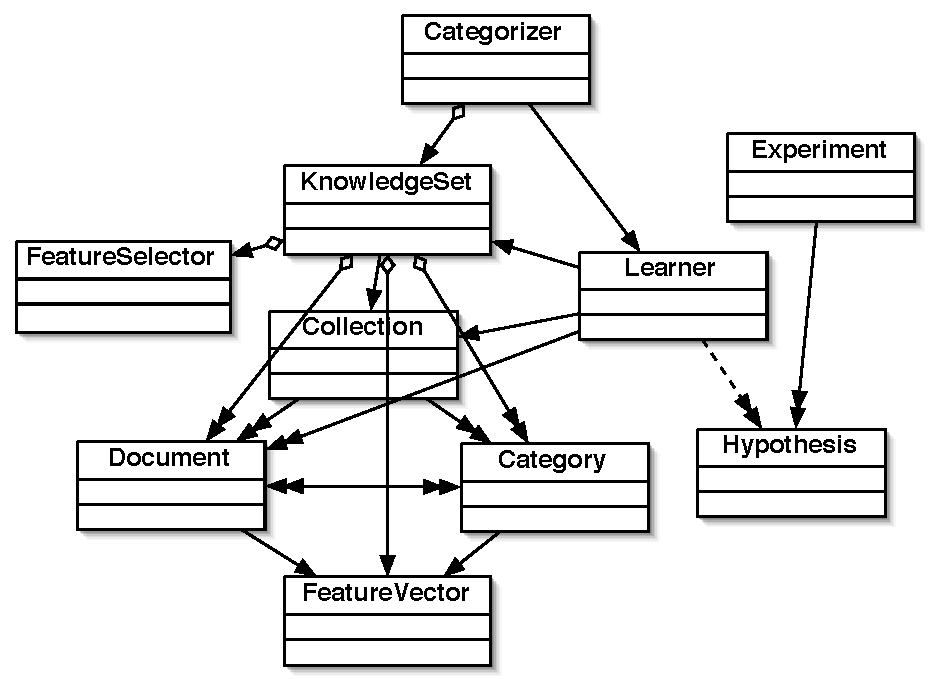
\includegraphics[width=\linewidth]{figures/classes-uml.pdf}
\caption{Class composition diagram for \aicat}
\label{classes-uml}
\end{figure}

Some examination of the basic relationships between classes and the
responsibilities of each class is helpful before looking at the design
in more detail.  The major classes in the \aicat\ framework
are:

\begin{description}

\item[KnowledgeSet]

The \class{KnowledgeSet} class represents a set of processed documents, a set
of categories, and a many-to-many mapping between the two sets.
Processing may involve tokenization, stopword removal, linguistic
stemming, feature selection, and vector weighting.  Note that the term
``knowledge set'' is somewhat unique to this project.

A \class{KnowledgeSet} contains references to many \class{Document} objects and
\class{Category} objects.  It uses \class{Collection} objects to instantiate \class{Document}
and \class{Category} objects.  It uses a \class{FeatureSelector} object to perform
feature selection.  It also contains a \class{FeatureVector} object
representing the features present in all documents.

\item[FeatureSelector]

Feature selection is performed by subclasses of the \class{FeatureSelector}
class.  Each \class{KnowledgeSet} object contains a \class{FeatureSelector}
object--the \class{KnowledgeSet} provides the information necessary to do
feature selection, and the \class{FeatureSelector} performs the desired
feature selection algorithm.

\item[Collection]

Because data sets in text categorization may be very large, and
because their documents may exist in several different underlying
storage mechanisms (e.g. as files in a filesystem, sections of a
larger XML file, or fields in a database), a \class{Collection} class provides
an abstract interface to a set of stored documents, together with a
way to iterate through the set and return \class{Document} objects.

A \class{Collection} object may be used in several contexts within the
framework.  For instance, a \class{KnowledgeSet} instantiates its Document and
\class{Category} objects through a \class{Collection} object.  A \class{Learner} object may
also mass-categorize the \class{Documents} in a \class{Collection} object.

\item[Document]

Each text document is represented by a \class{Document} object, or an object
of one of its subclasses.  Each document class contains methods for
turning document data into a \class{FeatureVector}.  Each document also has
a method to report which categories it belongs to.

\item[Category]

Each category is represented by a \class{Category} object.  Its main purpose
is to keep track of which documents belong to it, though it also
contains methods for examining statistical properties of an entire
category.

\item[Learner]

The abstract \class{Learner} class provides an interface to train on a
set of pre-categorized documents and subsequently categorize
previously unseen \class{Document} objects.  Its
concrete subclasses implement specific categorization algorithms like
Naive Bayes, SVM, Decision Tree, and so on.

\item[FeatureVector]

Most categorization algorithms don't deal directly with documents'
data, they instead deal with a \emph{vector representation} of a
document's features.  Most often, documents are represented using the
``Bag of Words'' model \cite{XXX}, i.e. a non-ordered, weighted set of
features.  The \class{FeatureVector} class provides an interface to the
operations one may perform on these vector representations, such as
querying features' presence or absence in a document, adding vectors
to each other, and so on.

\item[Hypothesis]

The result of asking a \class{Learner} to categorize a previously unseen
document is a \class{Hypothesis} object.  It may be queried for information
about which categories were assigned, which category was the single
most appropriate category, what scores were assigned to each category,
and so on.

\item[Experiment]

The \class{Experiment} class can examine the results of many categorization
decisions (i.e., many \class{Hypothesis} objects) and may be queried for
aggregate information about the results.  This is often used in order
to determine the quality (as measured by precision, recall, error,
etc.) of a \class{Learner} on a collection of test documents.

\item[AI::Categorizer]

An umbrella class \aicat\ sits above the rest of the classes,
providing a convenient interface to a complete system for text
categorization.  Most applications built using the framework will
instantiate an object of this class.  Note that the term \aicat\ can
refer either to the framework as a whole, or to the umbrella class.
The distinction will be made clear in the text where it is necessary
to do so.

\end{description}

\section{Design Patterns in \aicat}

The real power and intellectual content of any framework lies not in
the design of its individual classes, but in the interfaces between
the classes and the way objects collaborate to solve problems in the
framework's application domain. \cite[p. 31]{fayad:99} These
relationships can be quite complicated and difficult to explain, yet
understanding them is essential to understanding the framework.

In order to shed light on the design of complex object-oriented
systems, many researchers and software developers have tried to
standardize language and notation for class and object relationships.
There is as yet no universally accepted terminology for describing
these relationships, but one common practice is to use so-called
``design patterns'' to provide a baseline grammar for discussing
commonly seen patterns of cooperation in object-oriented
design. \cite[p. 3]{gamma:95} The design patterns do not provide
prescriptions for software design, but rather descriptions of best
practices in common situations.  Most design patterns in
\cite{gamma:95} include discussions of various trade-offs in their
application, indicating that a design pattern is actually a family of
similar solutions to a problem, not one rigid solution.

In this section, certain important local structures in the \aicat\
framework design will be discussed using the language of design
patterns.  The ``Iterator,'' ``Composite,'' ``Adapter,'' ``Strategy,''
and ``Factory Method'' patterns are discussed, and specific examples
from \aicat\ show how they are applied within the framework.  These
are not by any means the only instances of common design patterns in
the framework, nor do the specific patterns in \cite{gamma:95} provide
a complete catalog of all possible patterns in software.  This
discussion also does not give complete coverage to all design-related
issues involved in \aicat.  But patterns often provide a starting
point for design discussion, and their use has been found beneficial
in many diverse arenas \cite{granlund:99}, so they are used here in
the hope that they clarify the important design issues.

\subsection{Iterator}

The Iterator pattern provides ``a way to access the elements of an
aggregate object sequentially without exposing its underlying
representation.'' \cite[p. 257]{gamma:95} Its main purpose is to
decouple the traversal process on an object's aggregate members from
the object's internal data structure implementation.  In this way,
clients can iterate through aggregate objects without knowing the
objects' internal structure.

In the \aicat\ framework, it is often necessary to iterate
through collections of documents and perform some action on them.  For
example, the documents may form a training set for a \class{Learner} to base a
model on, or they may form a test set on which to evaluate the model.

The \class{Collection} class implements the Iterator pattern
\cite[p. 257]{gamma:95} over documents in the framework.  Figure
\ref{Iterator-collection} shows the main relationships involved in
this pattern.

\begin{figure}
\includegraphics[width=\linewidth]{figures/Iterator.pdf}
\caption{The Iterator pattern in the \class{Collection} class}
\label{Iterator-collection}
\end{figure}


\cite[p. 259]{gamma:95} suggests that the most common reasons for
using a formal custom iterator are:

\begin{itemize}

\item to access an aggregate object's contents without exposing its
internal representation.

\item to support multiple traversals of aggregate objects.

\item to provide a uniform interface for traversing different
aggregate structures.

\end{itemize}

The first and third reasons are most germane to the document iteration
process.  As explained in section \ref{Document storage}, it is
important that the framework can directly import documents from their
various underlying storage mechanisms in order to prevent unnecessary
duplication of data.  In order to hide the details of the storage
mechanism from the rest of the framework, a \class{Collection} object
retrieves documents from several storage mechanisms and returns them
as \class{Document} objects.  It provides a unified interface to iteration
over stored documents so that the various classes that need to perform
this iteration (chiefly \class{Learner} and \class{KnowledgeSet}) don't need to be
aware of storage issues.  In this sense, the ``internal
representation'' of the aggregate structure is often external to the
framework itself--it may be files in a filesystem, entries in a
database, records in an XML document, or another mechanism.

In addition to providing a generic interface to a stored collection of
documents, the Iterator pattern allows clients of the \class{Collection} class
to use memory efficiently.  A \class{Collection} object will typically defer
creation of its \class{Document} objects until its client calls its
\method{next} method.  In this way, the \class{Collection} doesn't store all
the \class{Document} objects in memory simultanously--if the client needs to do so,
it can, or it can merely query properties of each document and dispose
of them in turn.

Note that the \class{Collection} class defines a \method{next} method,
but no \method{previous} method.  This is largely because common
document storage mechanisms like filesystems or databases typically
only have one-directional iterators.  Insisting that
\class{Collection} classes needed to implement a \method{previous}
method to support bi-directional iteration would impose an
unreasonable burden on them.

In order to decouple the storage mechanism from the internal format of
documents (see section \ref{Document format}), \class{Collection}
classes can cooperate with any subclass of the \class{Document} class.
The client of the \class{Collection} class informs it that it should
instantiate documents using a certain \class{Document} subclass.
Since the \class{Document} subclasses share a common interface, \class{Collection}
may remain ignorant of all internal document formatting issues,
passing data to the proper constructors in order to instantiate
\class{Document} objects.


\subsection{Composite}

The Composite pattern ``lets clients treat individual objects and
compositions of objects uniformly.'' \cite[p. 163]{gamma:95} It is
often used to represent trees or other data structures in which the
form of a subset of the structure is not qualitiatively different from
the form of the entire structure.  In simple terms, this means that
the same kinds of operations--iteration over subnodes, inspection of
the root node, and so on--can be performed on the entire tree, a
subtree, or even a single node.

In fact, the Composite pattern does not apply only to tree
structures.  It applies whenever a self-similarity exists between the
whole and the parts in a part-whole hierarchy.

One instance of this kind of structure in Text Categorization is in
so-called ``ensemble learners,'' also known as ``classifier
committees.''  An ensemble learner is a categorizer that combines the
results of a set of other categorizers in some way to arrive at a
categorization result of its own. \cite[p. 30]{sebastiani:02} Often,
an ensemble learner may outperform each of its constituent members on
the general categorization task.  \cite{tumer:98}

To implement ensemble learners within \aicat, the Composite
pattern may be applied to the \class{Learner} class to create a
\ensemble\ subclass.  Figure \ref{Composite-ensemble}
shows the classes participating in this pattern.

\begin{figure}
\includegraphics[width=\linewidth]{figures/Composite.pdf}
\caption{The Composite pattern in the \ensemble\ class}
\label{Composite-ensemble}
\end{figure}

Since \ensemble\ is a subclass of the abstract
\class{Learner} class, it conforms to the \class{Learner} interface.
This is crucial to implementation of the Composite pattern--it means
that clients may use the \ensemble\ class without
knowing that it implements an ensemble learner behind the scenes.  In
this way, transparent ensemble learning is achieved through
polymorphism.

According to \cite[p. 30]{sebastiani:02}, ensemble learning techniques
can be specified by (1) a set of individual learners (the ``members''
in Figure \ref{Composite-ensemble}), and (2) a mechanism for combining
the output of the individual learners.  The \ensemble\
class can provide generic support for creating the member learners of
the ensemble, but the combination mechanism may take many different
forms.  Such algorithms are an active area of Machine Learning
research.  As such, \ensemble\ may be subclassed in
order to implement different combination mechanisms.  Since these
subclasses implement the combination algorithm in different ways, they
may themselves be seen as carrying out a Strategy pattern (see section
\ref{Strategy}).


\subsection{Adapter}

The Adapter pattern ``converts the interface of a class into another
interface clients expect.'' \cite[p. 139]{gamma:95} It is commonly
used when an existing resource provides the functionality necessary
for a certain task, but the interface of that resource doesn't match
the interface necessary for the environment in which that task must be
performed.  For example, a framework may require that a particular
role is implemented by subclasses of a certain abstract class.  This
helps unify functionality by taking advantage of polymorphic
abstraction. \cite[p. 5]{fayad:99} That functionality may already be
present in an existing body of code outside the framework.  An Adapter
can help bridge the gap between the two code bodies by letting the
external code function inside the framework.\footnote{An Adapter may
sometimes be called a Wrapper.  Both terms will be used in this
discussion.}

Many developers in the text categorization community create their
software as demonstrations of novel algorithms, or as stand-alone
libraries that implement one small part of the overall text
categorization task.  The majority of cutting-edge research will be
implemented in this way, if a public implementation is available at
all.  In order to leverage this work for a categorization framework,
some adaptation is invariably necessary.  Unless a developer happened
to be using \aicat\ as a development environment, her implementation
will not be directly usable as a framework element.  Thus Adapters
provide a mechanism for keeping the framework current with advances in
the field of text categorization.

\begin{figure}
\includegraphics[width=\linewidth]{figures/Adapter.pdf}
\caption{The Adapter pattern in the Learner class}
\label{Adapter-learner}
\end{figure}

Figure \ref{Adapter-learner} shows how the Adapter
pattern is present in \aicat's \class{Learner} class.  The abstract
\class{Learner} class specifies a common interface that all subclasses
must conform to.  Several of its concrete subclasses implement their
functionality using a framework-external resource.  For example,
\class{Learner::DecisionTree} uses the stand-alone module
\class{AI::DecisionTree} for implementation.  \class{Learner::Weka}
is a wrapper around the ``Weka'' Machine Learning system.
\class{Learner::SVM} is a wrapper around a framework-external
\class{Algorithm::SVM} module, which is itself a wrapper around the
\texttt{libsvm}\cite{libsvm} C library.\footnote{Note that
\class{Learner::SVM}, Weka, and \texttt{libsvm} are not part of the
contributed work of this thesis, as they are written by other authors.}

Note that these four Adapter examples exhibit three very different
applications of the Adapter pattern.  \class{Learner::DecisionTree}
exhibits a very straightforward Adapter usage as presented in
\cite{gamma:95}--an existing standalone class exists that implements the
needed functionality, and its interface is adapted to the framework
requirements by a simple wrapping subclass.  The \class{Learner::SVM}
wrapper is also fairly straightforward.  However, the other two
wrappers exhibit well the highly heterogeneous nature of the text
categorization domain.  The main reason for the adaptation in the
\class{Algorithm::SVM} class is to provide a Perl interface to a C
library.  The \class{Learner::Weka} adapter combines language
adaptation (in this case, Java to Perl) with functionality
transformation (mapping Weka's methods to the required \class{Learner}
interface).

Adapters can create design flexibility.
The current implementation of \class{Learner::Weka} interfaces with
Weka through its command-line interface, but this is not a design
constraint.  Future implementations may embed the Weka system inside
the \class{Learner::Weka} module for reasons of efficiency or platform
compatibility.  Because this interface is hidden using an Adapter
pattern, the implementation may be changed freely.

The differences in interfaces between the Adapter and the Adaptee may
be merely historical, or they may reflect different needs in different
domains.  The Adapter must conform to the interface of its abstract
superclass, which is typically designed to be independent of subclass
abilities and implementations.  The Adaptee may be designed for use in
a different arena, with extra functionality, or an interface that
takes full advantage of its capabilities.

Using Adapters may bring major benefits in the area of reusability.
Obviously, classes won't have to be re-implemented if the
functionality can be adapted from an existing implementation.  Second,
and perhaps more importantly, classes initially implemented for a
framework may be converted into Adaptee classes, usable in isolation.
This can bring them better exposure in other projects and thus more
feedback, maturing them quickly.  This can be a major win, because
iteration is considered a limiting factor in framework development
\cite[p. 75]{fayad:99}, and any process that speeds up maturity in
framework components can have a large impact.  Adapters can also force
a more robust encapsulation of design in the Adaptee, bringing
benefits in the conceptual and technical segmentation of the
framework.

\subsection{Strategy}
\label{Strategy}

The Strategy pattern defines ``a family of algorithms, encapsulates
each one, amd makes them interchangeable.'' \cite[p. 315]{gamma:95}
It is used when a domain task needs to be carried out, but there may
be several ways to carry out that task, and it is important to let the
user or client choose from among these alternatives.

An important concept in the Strategy pattern is that of ``behavior.''
In \cite{gamma:95}, the Strategy pattern is recommended when ``many
related classes differ only in their behavior.''  In this context, a
distinction is made between an algorithm's purpose and its behavior.
For example, a set of algorithms for finding line-break points in text
paragraphs have a common purpose (to accomplish the line-breaking
task), but they may carry out their task in different ways.  The
algorithms may make different trade-offs in terms of speed and memory,
or they may try to optimize different aspects of the task.  Since it
is impossible to satisfy all clients in all situations with a single
choice of algorithm, it is desirable to encapsulate each algorithm in
a class that can be chosen or extended by the client.

The field of text categorization has several natural applications for
the Strategy pattern.  One of the primary concerns of most TC
researchers is the development of novel algorithms for various aspects
of the categorization task, so it is essential for these algorithms to
be easy to vary in a categorization framework.  In the language of
\cite{fayad:99}, these algorithms are framework ``hot spots.''

The most obvious Strategy application in \aicat\ is the
\class{Learner} class and its subclasses.  These classes all have a
common task to perform, that of training a categorizer and
categorizing unseen documents.  The various subclasses represent very
different ways to accomplish that task.  Importantly, the results of
the task, and not just the internal mechanism that performs it, may be
different depending on which \class{Learner} subclass is used.

\begin{figure}
\includegraphics[width=\linewidth]{figures/Strategy.pdf}
\caption{The Strategy pattern in the Learner class}
\label{Strategy-learner}
\end{figure}

Figure \ref{Strategy-learner} shows how the Strategy pattern appears
in the \class{Learner} class and its subclasses.  Three concrete
subclasses are shown that implement specific Machine Learning
algorithms (see Figure \ref{inheritance-uml} for other \class{Learner}
subclasses currently implemented).  From the point of view of the
client \aicat\ object, all \class{Learner}s have the same interface,
and may therefore be treated uniformly.  The framework user or
application designer, however, may choose judiciously among subclasses
depending on the particular needs of the application.  Customizability
of the Machine Learning algorithm is of paramount importance to the
framework, since it would be useless to researchers if this were not
the case.

Each \class{Learner} subclass must implement the abstract
\method{train} and \method{categorize} methods in order to perform the
two essential tasks of any \class{Learner}.  The \method{train} method
examines a \class{KnowledgeSet} object and builds an internal (and
opaque) model that will be used to categorize future documents.  The
\method{categorize} method takes a \class{Document} object as an
argument and returns a \class{Hypothesis} object representing the
outcome of categorization based on the model.

\begin{figure}
\includegraphics[width=\linewidth]{figures/Strategy-feasel.pdf}
\caption{The Strategy pattern in the FeatureSelector class}
\label{Strategy-feasel}
\end{figure}

Another application of the Strategy pattern is shown in Figure
\ref{Strategy-feasel}.  Here, the varying algorithm performs
feature selection, another framework hot spot.  There has been much
activity in current research on improving feature selection for
different scenarios \cite{yang:01,yang:97}, so customization in this
area is also essential.

To perform feature selection, a \class{KnowledgeSet} object invokes
either the \method{select\_features} or \method{scan\_features} method
of the \class{FeatureSelector} object, depending on whether a complete
\class{KnowledgeSet} or a \class{Collection} object should be
examined.  Examining a \class{Collection} iteratively requires less
memory because the documents don't have to be loaded into memory all
at once, but it requires a separate pass through the data.  The choice
of which method to run is made in response to user specification.

Because \method{select\_features} and \method{scan\_features} are
virtual methods in the parent class, any concrete subclass must
implement these methods according to the particular algorithm the
subclass represents.  As of this writing, only the
\class{FeatureSelector::DocFrequency} subclass is implemented, but
the other subclasses in the diagram are planned.


\subsection{Factory Method}

XXX need to write \ldots


\section{Specifying framework relationships}

In object-oriented programming, the language itself usually provides
first-class support for describing inheritance relationships between
classes.  For instance, a C++ or Java \texttt{class} declaration lists
its superclasses explicitly, and Perl specifies inheritance via each
class's \texttt{@INC} array.  Because inheritance is directly
implemented by the language, it is easy for framework users to
understand inheritance relationships, and these relationships are
expressed straightforwardly in the framework code.\footnote{Contrast
this with object-oriented programming in languages like C that don't
have inherent OO support, where understanding the inheritance
structures can be much more challenging.\cite[p. 7]{fayad:99}}

However, effective frameworks have many complicated interrelationships
besides inheritance.  These need to be specified somehow in the
implementation language of the framework so that the proper
relationships are created, and they need to be specified in
documentation so that users of the framework understand the structure
of the software they're using.

In addition, as explained in Section \ref{class-overview}, these
relationships are typically much more important and enlightening to
users of the framework than the inheritance relationships.  It is
desirable to treat these relationships in a unified manner, so that
all identical collaborations in the framework are specified in and
will function in similar ways.\cite[p. 13]{fayad:99}

Since Perl lacks first-class support for specifying patterns of
collaboration (as is the case with most common OO languages), a
language extension called \class{Class::Container} has been employed
in the \aicat\ framework to unify these issues.  Using this extension,
each class explicitly
declares any other objects it cooperates with in certain types of
relationships.  Because these declarations are made explicitly and
don't just emerge from usage patterns in the implementation code,
certain types of functionality may be handled centrally and
consistently, greatly easing the burden of implementing these
relationships and aiding framework flexibility.

For example, XXX \ldots

\section{Limitations}

XXX Here, write about basic assumptions \aicat\ makes about the
general TC problem, and what happens when those assumptions aren't
true.  For example, structured feature vectors instead of flat,
non-bag-of-words, etc.

